\chapter{Реализация и экспериментальная проверка}

\begin{annotation}
	В данной главе приводятся детали разработки и экспериментальной проверки
	разработанной системы. Описан выбор инструментов, используемых для реализации
	программного обеспечения. Так же приводится выбор инфраструктурных решений,
	с учетом поставленных ранее системных и функциональных требований.
	Разработаны тестовые примеры для тестирования приложения
	и приведена оценка качества работы системы. Описаны состав и структура
	реализованного программного обеспечения.
\end{annotation}


% Недостаток ~- это то, что градиент не ходит по ансамблю, а только
% внутри одной модели. Возможно, если сделать из этого одну модель
% и изучить то, как будет работать в ней обратные связи, рекурентность,
% мы можем оптимизировать вычисления и процесс обучения.


\section{Выбор инструментальных средств}
\begin{annotation}
	В данном разделе обосновывается выбор инструментальных средств с учетом выдвинутых в 3
	главе требований к системе. Рассматриваются инструменты для обработки и хранения данных,
	для разработки backend и frontend части приложения.
\end{annotation}

% В этом разделе обосновывается выбор инструментальных средств; одним из критериев выбора могут быть какие-либо требования к разрабатываемой системе, и если этих требований много, они могут быть выделены в отдельный раздел, или же в приложение. Этот пункт не пишется, если в аналитической главе был раздел, посвященный сравнительному анализу и выбору инструментальных средств.

% В качестве системы, реализующей очереди, будет использован Python модуль aiotasks.
% Этот модуль позволяет в одном процессе запустить сразу несколько ассинхронных обработчиков задач.
% Если обработчики выполняют io-bound задачи (задачи, которые большую часть времени
% ждут операций ввода-вывода), такая архитектура может обрабатывать на порядки больше запросов,
% в сравнении с однопоточными обработчиками на io-bound классе задач.

% Для распараллеливания работы с данными и использовании аппаратных ускорений для умножений матриц
% для реализации модуля подсистемы обработки данных и подсистемы для вычисления нечеткой карты
% будет использоваться pytorch. Это фреймворк для работы с данными и созданию нейросетей.

% Кроме того, для работы с данными будет исползоваться Python-библиотека networkx. А для визуализации данных
% - matplotlib.


\section{Состав и структура реализованного программного обеспечения}
\begin{annotation}
	В данном разделе рассматривается состав и структура реализованного программного обеспечения.
	Приводятся характеристики разработанного программного продукта, возможности конфигурации отдельных
	компонент системы. Описано назначение исполняемых файлов, описаны требования к системному окружению.
\end{annotation}

% Нужно охарактеризовать реализованное ПО: является ли оно настольной программной для Windows, или веб-приложением в  форме сайта/веб-сервиса, или модулем/подключаемой библиотекой, или \dots. Также нужно перечислить, из чего оно  состоит: какие исполняемые файлы и их назначение, конфигурационные файлы, файлы баз данных, требования к программному  и аппаратному окружению, и т.п.

% Если реализованное приложение достаточно обширно, этот раздел может быть
% разделен на несколько: один с общим описанием, и по одному на подсистемы самого
% верхнего уровня.


% Разработанное программное обеспечение состоит из:
% \begin{itemize}
% 	\item Подсистемы скачивания данных
% 	\item Подсистемы обработки данных
% 	\item Подсистемы для построения когнитивных картирования
% 	\item Подсистемы общения с пользователем
% \end{itemize}

% Все подсистемы работают на удаленном сервере под управлением дистрибутива ОС Linux Ubuntu.


% \section{Основные сценарии работы пользователя}

% Нужно помнить, что пользователем может быть не только <<менеджер>> или <<человек в белом халате>>, но и другой программист. Последнее относится, в первую очередь, к реализованным библиотекам. Для <<обычных>> приложений нередко бывают пользователи нескольких категорий --- например, обычный пользователь и администратор. Для каждой категории нужно описать, как выполняются основные функции, предпочтительно, с помощью серии скрин-шотов. Однако считается плохим тоном вставлять длинную вереницу из скрин-шотов: если их много, большую часть нужно выносить в приложение. Для \textit{этого} раздела нормальной является плотность скрин-шотов из расчета: 1 страница скрин-шотов на 1-2 страницы текста.





\section{Разработка тестовых примеров}
\begin{annotation}
	В данном разделе описывается процесс тестирования разработанной системы.
	Описаны реализованные unit-тесты и описывается процесс функционального тестирования.
	Приводятся результаты тестирования. Проверка того, что система соответствует выдвинутым ранее требованиям.
	Производится оценка работы системы.
\end{annotation}
% Описываются наиболее характерные тестовые примеры, для прогона на интеграционных тестах. (Да, использование unit-тестирование --- это почти всегда хорошо, основное исключение составляют работы, в которых используемый инструментарий по какой-либо причине в принципе исключает такую возможность. Например, что-нибудь вроде Mathematica.)

% В этом же разделе могут приводится и результаты тестирования, включая таблицы и
% графики. Результаты тестирования могут быть вынесены в отдельный раздел, если
% много текстового материала и/или использована (не совсем) стандартная методика
% тестирования (описание которой также нужно привести).

% \textit{\textbf{Замечание.}} В ПЗ (как УИРа, так и ВКР) следует избегать ситуаций, когда значительную часть основного содержания составляют страницы с иллюстрациями и таблицами, особенно, если такие страницы следуют подряд. В основном тексте следует оставлять лишь самые основные таблицы и рисунки, а остальное --- выносить в приложение.


% \section{Сравнение реализованного программного обеспечения с существующими аналогами}

% В сравнении должно быть отражено, чем полученное ПО выгодно (и невыгодно) отличается от прочих ближайших аналогов. Практика показывает, что аналоги есть всегда. А если нет аналогов, значит есть частичные решения, которые реализуют какие-то части функционала вашей системы. Тут тоже может быть относительно много таблиц и графиков.

% В качестве тестовых данных были взяты данные из нового источника - lenta.ru.
% Были проанализированы данные с 2018-09-30 по 2018-12-14.

% Распределение количества постов по дням представлено на рис. \ref{pic:lenta_posts_by_day}

% \begin{figure}
% 	\begin{center}
% 		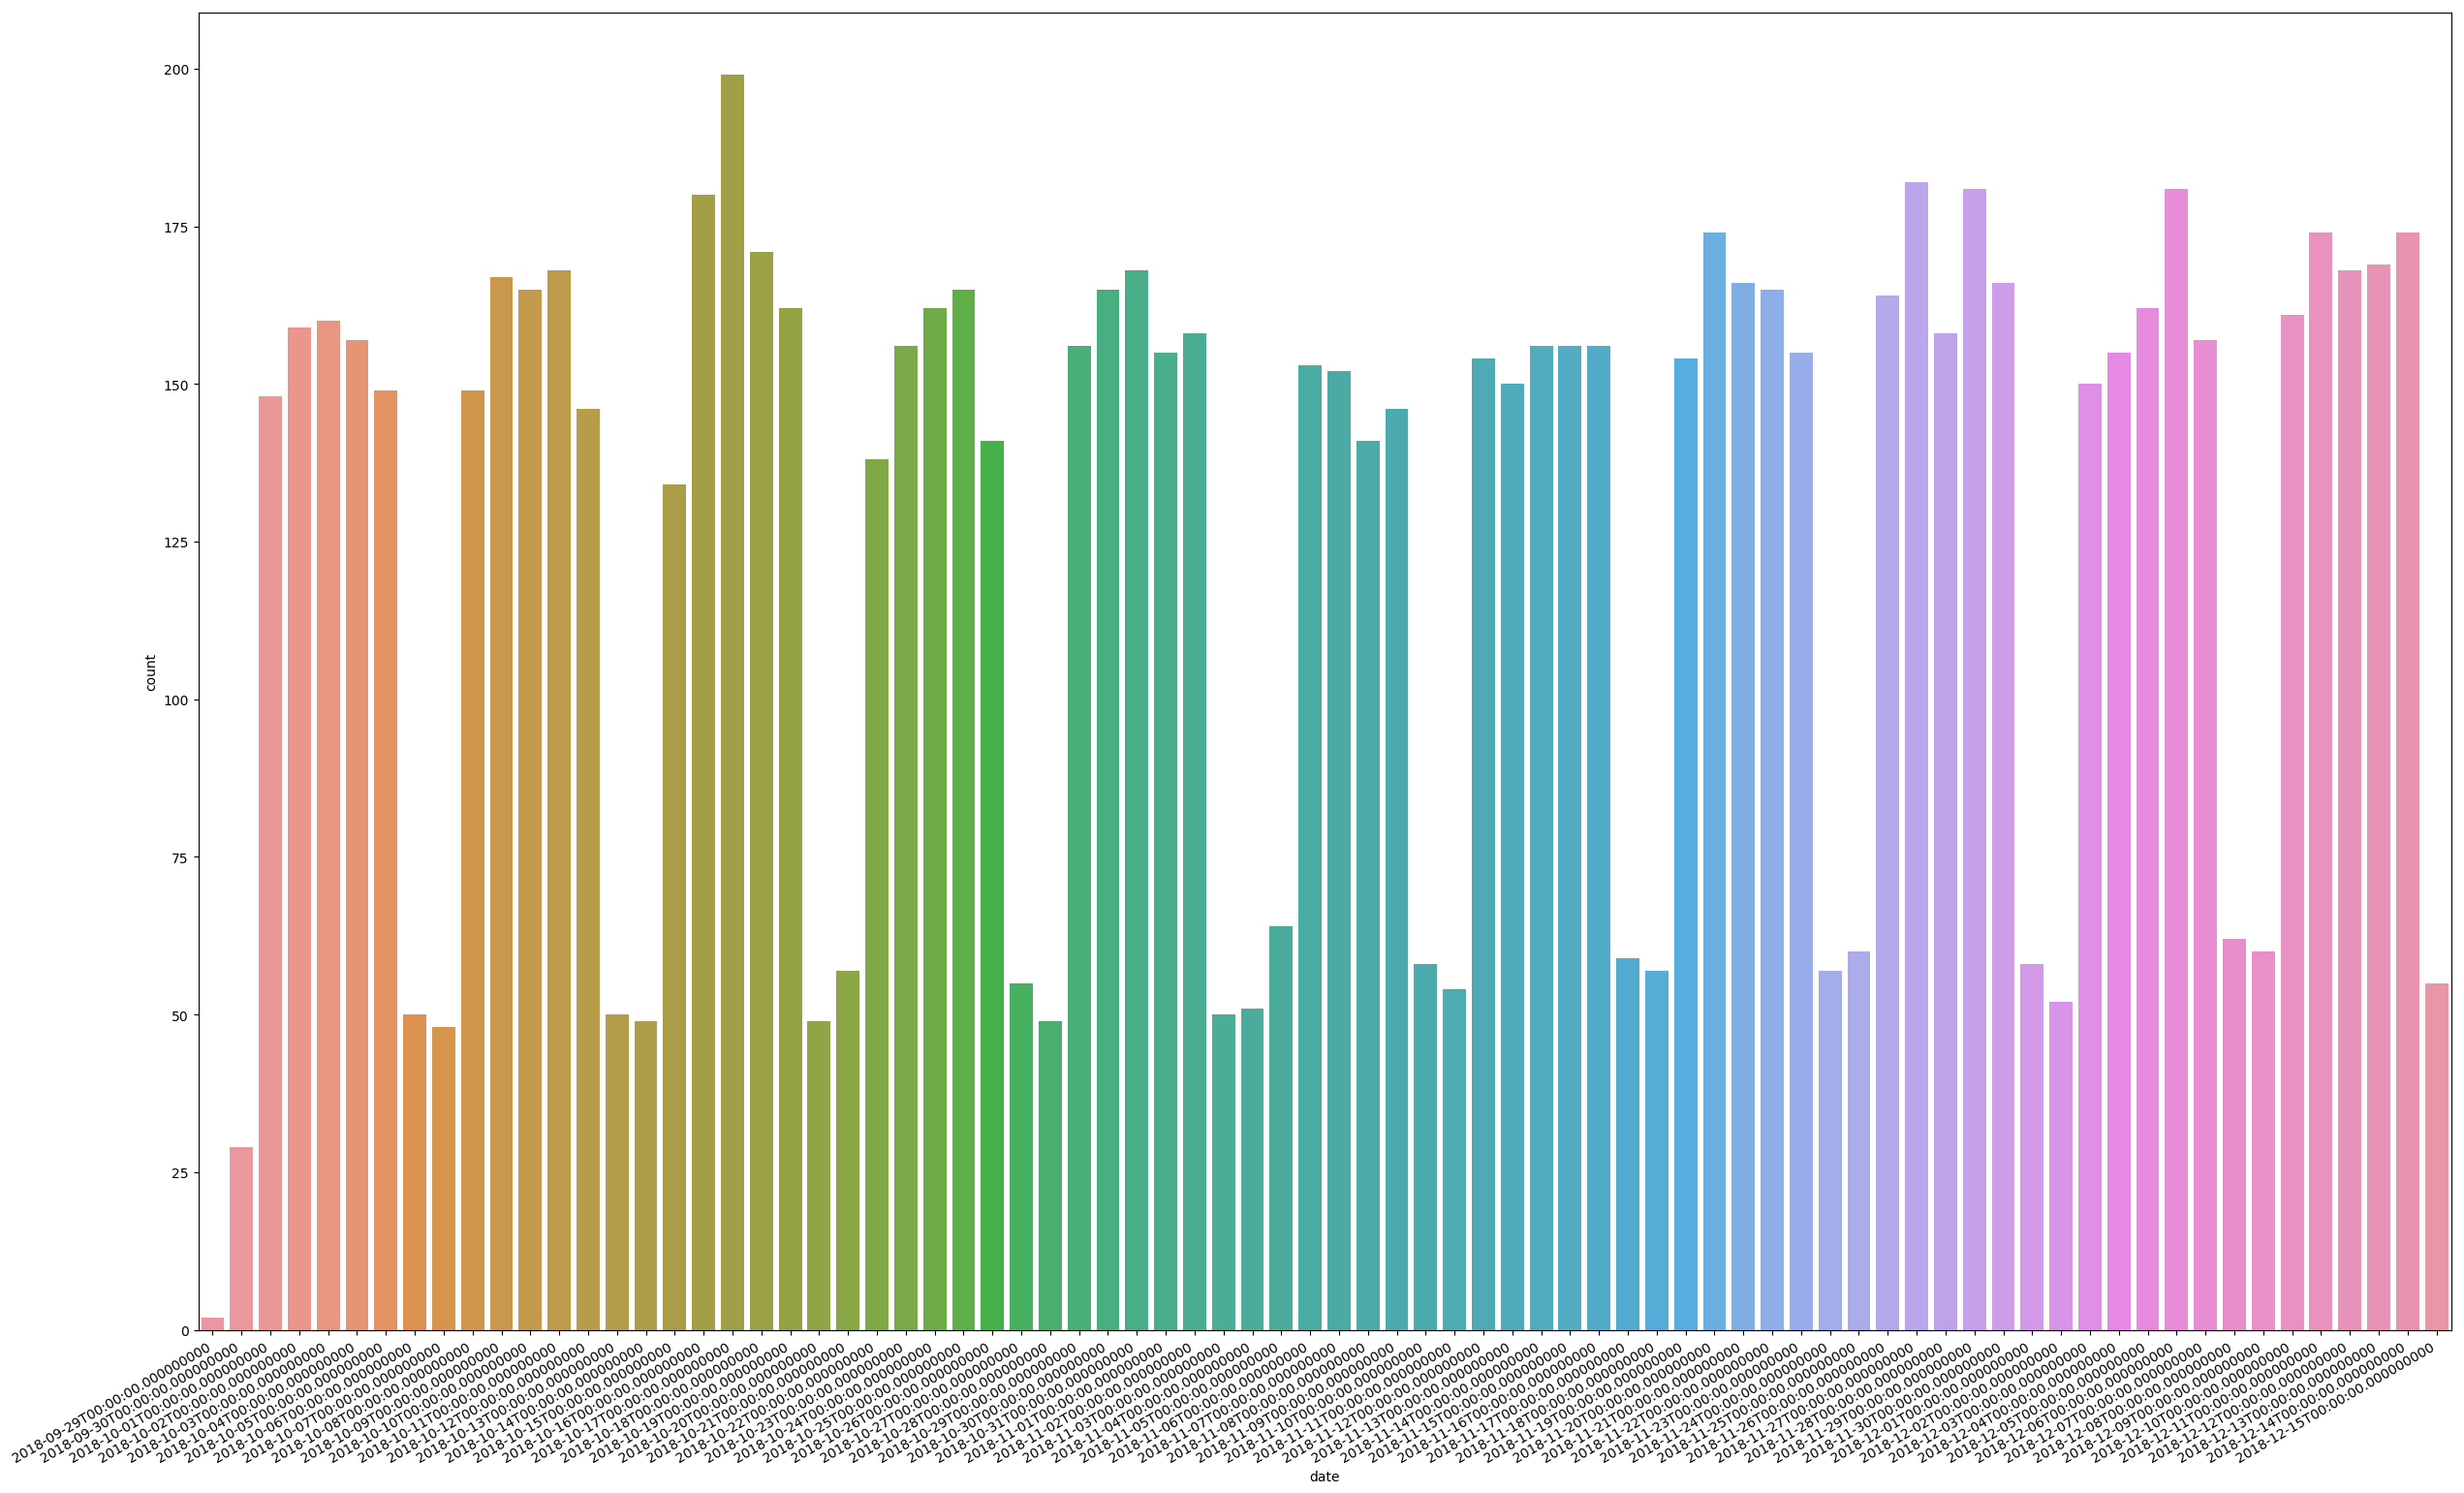
\includegraphics[width=.5\columnwidth]{./img/lenta_posts_by_day.png}%
% 	\end{center}

% 	\caption{Распределение количества постов по дням.}%
% 	\label{pic:lenta_posts_by_day}%
% \end{figure}


% \begin{table}
% 	\centering
% 	\begin{tabular}{|l|c|}
% 		\hline
% 		Название темы & Количество постов \\
% 		\hline
% 		Политика & 12529	\\
% 		Общество & 9092	\\
% 		Происшествия & 5913	\\
% 		Украина & 5425	\\
% 		Футбол & 4927	\\
% 		Госэкономика & 4212	\\
% 		Интернет & 3182	\\
% 		Следствие суд & 3064	\\
% 		Кино & 2942	\\
% 		Музыка & 2358

% 	\end{tabular}

% 	\caption{Наиболее обсуждаемые темы на lenta.ru за 2018-09-30 - 2018-12-14. Абсолютные значения}
% 	\label{tbl:top_tags}
% \end{table}

% \begin{table}
% 	\centering
% 	\begin{tabular}{|l|c|}

% 		\hline
% 		Название темы & Процент постов \\
% 		\hline

% 		Политика		& 13.20\%	\\
% 		Общество		& 09.58\%	\\
% 		Происшествия	& 06.23\%	\\
% 		Украина			& 05.71\%	\\
% 		Футбол			& 05.19\%	\\
% 		Госэкономика	& 04.43\%	\\
% 		Интернет		& 03.35\%	\\
% 		Следствие суд	& 03.22\%	\\
% 		Кино			& 03.10\%	\\
% 		Музыка			& 02.48\%

% 	\end{tabular}
% 	\caption{Наиболее обсуждаемые темы на lenta.ru за 2018-09-30 - 2018-12-14. Относительные значения}
% 	\label{tbl:top_tags_percent}
% \end{table}



% Количество постов по выходным заметно меньше, чем в будние дни.
% Для того, чтобы абсолютные колебания значений не влияли на значения концептов,
% для первого приближения возьмем значение концептов равным проценту тем, о которых пишут
% посты от общего числа тем. Так как это значение всегда положительное,
% мы должны взять такую функцию активации, в которой значения,
% близкие к нулю изменяются линейно. В данной работе был использован $ tanh(x) $ в качестве функции
% активации.

% Предположим, что каждый концепт оказывает влияние на каждый другой концепт с
% некоторым весом, нормально распределенным $ \sigma = 1, \mu = 0 $

% Темы с максимальным количеством постов за рассматриваемый период приведены в таблице \ref{tbl:top_tags}.
% Относительные значения этих парамтеров представлены в таблице \ref{tbl:top_tags_percent}

% На рис \ref{pic:nn_conc_history} изображены значения рассматриваемых концептов по месяцам.
% На 23 итерации карта обучалась. За 1 итерацию (с 23 по 24) значения концептов сошлись.
% Полученный результат выглядит адекватно.


% Для классического алгоритма пересчета концептов значения концептов представлены на рис \ref{pic:classic_conc_history}.
% Так как исходные веса были сгенерированы случайно, карта оказалась несбалансированной.
% В результате мы наблюдаем аномальный скачок всех значений концептов.
% Есл правильно подобрать веса и правильно сформировать связи между концептами,
% возможно добиться от карты более адекватного предсказания.


% Сама карта представлена на рис \ref{pic:nfcm}. Карта сходится за 11 итераций (23-34).


\section{Выводы}

В данной главе была реализована система для автоматического когнитивного картирования с использованием
методов нейронных сетей.
Также описаны инструменты, с помощью которых была реализована система.
Описана структура программного обеспечения, проведено тестирование разработанной системы.
На основе тестирования была дана оценка реализованной системе.

% В результате получили, что карта, построенная по классическому методу требует больше подготовки
% и больше ручной настройки, чем карта, построенная с помощью нейро-нечеткой системы.

% Значения, предсказанные картой с использованием нейро-нечеткой системы более адекватны, но
% с помощью классической карты теоретически тоже можно добиться такого результата. Но для этого потребуется
% больше ручной работы.

% Следует перечислить, какие практические результаты были получены, а именно: какое программное или иное обеспечение было создано. В число результатов могут входить, например, методики тестирования, тестовые примеры (для проверки корректности/оценки характеристик тех или иных алгоритмов) и др. По каждому результату следует сделать вывод, насколько он отличается от известных промышленных аналогов и исследовательских прототипов.

